\documentclass{article}
\usepackage[margin=1in]{geometry}
\usepackage{tikz}
\usetikzlibrary{positioning}

\begin{document}

\begin{center}
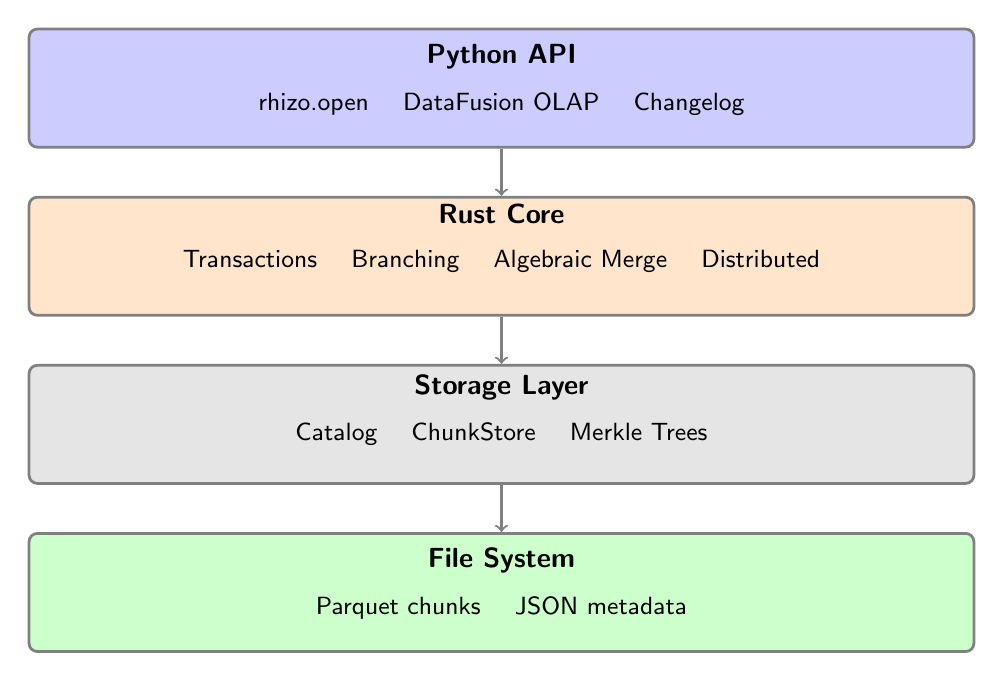
\begin{tikzpicture}[
    layer/.style={
        rectangle,
        rounded corners=3pt,
        minimum width=12cm,
        minimum height=1.5cm,
        draw=gray,
        line width=1pt,
        font=\sffamily
    },
    arrow/.style={
        ->,
        thick,
        gray
    }
]

% Python API Layer
\node[layer, fill=blue!20] (python) at (0,0) {};
\node[font=\sffamily\bfseries] at (0,0.4) {Python API};
\node[font=\sffamily\small] at (0,-0.2) {rhizo.open \quad DataFusion OLAP \quad Changelog};

% Rust Core Layer
\node[layer, fill=orange!20, below=0.6cm of python] (rust) {};
\node[font=\sffamily\bfseries] at (0,-2.0+0.4) {Rust Core};
\node[font=\sffamily\small] at (0,-2.0-0.2) {Transactions \quad Branching \quad Algebraic Merge \quad Distributed};

% Storage Layer
\node[layer, fill=gray!20, below=0.6cm of rust] (storage) {};
\node[font=\sffamily\bfseries] at (0,-4.2+0.4) {Storage Layer};
\node[font=\sffamily\small] at (0,-4.2-0.2) {Catalog \quad ChunkStore \quad Merkle Trees};

% File System Layer
\node[layer, fill=green!20, below=0.6cm of storage] (fs) {};
\node[font=\sffamily\bfseries] at (0,-6.4+0.4) {File System};
\node[font=\sffamily\small] at (0,-6.4-0.2) {Parquet chunks \quad JSON metadata};

% Arrows
\draw[arrow] (python.south) -- (rust.north);
\draw[arrow] (rust.south) -- (storage.north);
\draw[arrow] (storage.south) -- (fs.north);

\end{tikzpicture}
\end{center}

\end{document}
